\appendix 
\section*{Appendix I: Tables and Figures}
\begin{table}[H]																				
\tiny																				
  \centering																				
\captionsetup{width=.95\textwidth}																				
 \caption{\textbf{Descriptive Statistics}}  																				
 \label{summary-stats}																				
\caption*{This table presents descriptive statistics on uncertainty and firm characteristics.  Data span all stocks listed on the NYSE, NASDAQ, or American Stock Exchange (AMEX) and all industries over the years 1994 to 2017.

$AGE$ is the number of years the firm appears in Compustat.																				
$TURNOVER$ is the ratio of monthly trading volume to number of shares outstanding.																				
$RETURN$ is the stock return over the preceeding year.																				
$PRICE$ is the average daily stock price over the preceeding year.																				
$ASSETS$ is the natural logarithm of the book value of assets.																				
$MVE$ is the natural logarithm of market capitalization.																				
$NANALYSTS$ is number of analysts following the firm.																				
$PE$ is the forward price-to-earnings ratio, computed as the current price divided by the 1-year-ahead consensus analyst forecast for the firm.																				
$BASPREAD$ is the average bid-ask spread.																				
$SP500$ an indicator variable for whether or not the firm is in the S\&P 500.																				
$DIV$ is the dividend yield .																				
The ratio of the book value of total debt to assets ($LEVERAGE$.)																				
Tobin's $q$ ($Q$), calculated as in \cite{chungpruitt1994}.																				
Return on assets  ($ROA$)--the ratio of net income to the book value of total assets.																				
$LOSS$ is a dummy variable equal to one if $ROA$ is less than zero.																				
The level of asset tangibility ($TANG$), calculated as in \cite{almeidacampello2007}. All variables are winsorized at the 1\% and 99\% level. Final sample consists of 26,014 firm-year observations.}																				
    \begin{tabular}{rrrrrrrrrr}																				
    \toprule																				
          &       &       & \multicolumn{7}{c}{Percentile} \\																				
    \cmidrule{4-10}																				
    \multicolumn{1}{c}{Variable} & \multicolumn{1}{c}{Mean} & \multicolumn{1}{c}{Std Dev} & \multicolumn{1}{c}{1st} & \multicolumn{1}{c}{5th} & \multicolumn{1}{c}{25th} & \multicolumn{1}{c}{50th} & \multicolumn{1}{c}{75th} & \multicolumn{1}{c}{95th} & \multicolumn{1}{c}{99th} \\ \hline																				
\multicolumn{1}{l}	{AGE}	&	20.648	&	15.278	&	2.998	&	4.999	&	9.002	&	16.000	&	26.001	&	55.001	&	63.001	\\
\multicolumn{1}{l}	{AT}	&	3,577.017	&	9,129.440	&	19.662	&	41.621	&	178.232	&	611.070	&	2,350.677	&	17,716.150	&	62,404.883	\\
\multicolumn{1}{l}	{BASPREAD}	&	0.001	&	0.006	&	0.000	&	0.000	&	0.000	&	0.000	&	0.000	&	0.000	&	0.044	\\
\multicolumn{1}{l}	{BHR}	&	0.168	&	0.569	&	-0.761	&	-0.558	&	-0.172	&	0.082	&	0.369	&	1.207	&	2.760	\\
\multicolumn{1}{l}	{DIV}	&	1.545	&	5.372	&	0.000	&	0.000	&	0.000	&	0.000	&	0.465	&	8.019	&	40.850	\\
\multicolumn{1}{l}	{LEVERAGE}	&	0.191	&	0.184	&	0.000	&	0.000	&	0.006	&	0.157	&	0.315	&	0.548	&	0.702	\\
\multicolumn{1}{l}	{MVE}	&	3,920.795	&	10,981.519	&	19.168	&	47.306	&	218.759	&	677.059	&	2,399.036	&	17,677.582	&	82,215.576	\\
\multicolumn{1}{l}	{ANALYSTS}	&	6.692	&	6.992	&	0.000	&	0.000	&	1.000	&	5.000	&	10.000	&	22.000	&	30.000	\\
\multicolumn{1}{l}	{PE}	&	20.887	&	48.692	&	-163.572	&	-28.555	&	8.321	&	16.716	&	27.775	&	85.831	&	288.892	\\
\multicolumn{1}{l}	{PRICE}	&	25.695	&	22.691	&	2.126	&	3.451	&	9.016	&	19.088	&	35.088	&	70.449	&	121.255	\\
\multicolumn{1}{l}	{Q}	&	1.767	&	1.379	&	0.402	&	0.587	&	0.903	&	1.310	&	2.090	&	4.685	&	8.116	\\
\multicolumn{1}{l}	{ROA}	&	0.012	&	0.147	&	-0.643	&	-0.297	&	-0.009	&	0.040	&	0.082	&	0.175	&	0.307	\\
\multicolumn{1}{l}	{SP500}	&	0.147	&	0.354	&	0.000	&	0.000	&	0.000	&	0.000	&	0.000	&	1.000	&	1.000	\\
\multicolumn{1}{l}	{TANG}	&	0.499	&	0.186	&	0.000	&	0.189	&	0.387	&	0.501	&	0.601	&	0.837	&	0.948	\\
\multicolumn{1}{l}	{TURNOVER}	&	9.372	&	8.013	&	0.526	&	1.299	&	4.038	&	7.150	&	12.055	&	25.348	&	45.681	\\
\multicolumn{1}{l}	{LOSS}	&	0.276	&	0.447	&	0.000	&	0.000	&	0.000	&	0.000	&	1.000	&	1.000	&	1.000	\\
    \bottomrule																				
    \end{tabular}																				
\end{table} 
\newpage
\begin{sidewaystable}[H]
\tiny
\centering
\captionsetup{width=.95\textwidth}		
\caption{\footnotesize Correlation matrix of dependent variable, independent variable, and controls.\\
Labels are:(1) $AGE$; (2) $AT$; (3) $BASPREAD$; (4) $RETURN$; (5) $DIV$; (6) $LEVERAGE$; (7) $MVE$; (8) $NANALYSTS$; (9) $PE$; (10) $PRICE$; (11) $Q$; (12) $ROA$; (13) $SP500$; (14) $TANG$; (15) $TURNOVER$; (16) $LOSS$; (17) $NUM\_UNC$; (18) $PCT\_UNC$.\\
$AGE$ is the number of years the firm appears in Compustat.
$TURNOVER$ is the ratio of monthly trading volume to number of shares outstanding.
$RETURN$ is the stock return over the preceeding year.
$PRICE$ is the average daily stock price over the preceeding year.
$ASSETS$ is the natural logarithm of the book value of assets.
$MVE$ is the natural logarithm of market capitalization.
$BASPREAD$ is the average bid-ask spread.
$SP500$ an indicator variable for whether or not the firm is in the S\&P 500.
$DIV$ is the dividend yield .
The ratio of the book value of total debt to assets ($LEVERAGE$.)
Tobin's $q$ ($Q$), calculated as in \cite{chungpruitt1994}.
Return on assets  ($ROA$)--the ratio of net income to the book value of total assets.
$LOSS$ is a dummy variable equal to one if $ROA$ is less than zero.
The level of asset tangibility ($TANG$), calculated as in \cite{almeidacampello2007}. 
$NANALYSTS$ is the number of analysts following the firm.
$PE$ is the \emph{forward} price-to-earnings ratio computed as the current price divided by the one-year-ahead consensus analyst forecast.
All variables are winsorized at the 1\% and 99\% level.}\label{corr}
\begin{tabular}{rlllllllllllllllllll}
  \hline
% Fill in formatted numbers here
		&	(1)	&	(2)	&	(3)	&	(4)	&	(5)	&	(6)	&	(7)	&	(8)	&	(9)	&	(10)	&	(11)	&	(12)	&	(13)	&	(14)	&	(15)	&	(16)	&	(17)	&	(18)\\
	\hline	&		&		&		&		&		&		&		&		&		&		&		&		&		&		&		&		&		&	\\
AGE	(1)	&	1	&	 	&	 	&	 	&	 	&	 	&	 	&	 	&	 	&	 	&	 	&	 	&	 	&	 	&	 	&	 	&	 	&	 \\
AT	(2)	&	0.381	&	1	&	 	&	 	&	 	&	 	&	 	&	 	&	 	&	 	&	 	&	 	&	 	&	 	&	 	&	 	&	 	&	 \\
BASPREAD	(3)	&	0.013	&	-0.227	&	1	&	 	&	 	&	 	&	 	&	 	&	 	&	 	&	 	&	 	&	 	&	 	&	 	&	 	&	 	&	 \\
RETURN	(4)	&	0.052	&	0.035	&	0.007	&	1	&	 	&	 	&	 	&	 	&	 	&	 	&	 	&	 	&	 	&	 	&	 	&	 	&	 	&	 \\
DIV	(5)	&	0.445	&	0.487	&	-0.058	&	0.019	&	1	&	 	&	 	&	 	&	 	&	 	&	 	&	 	&	 	&	 	&	 	&	 	&	 	&	 \\
LEVERAGE	(6)	&	0.161	&	0.46	&	-0.015	&	-0.007	&	0.229	&	1	&	 	&	 	&	 	&	 	&	 	&	 	&	 	&	 	&	 	&	 	&	 	&	 \\
MVE	(7)	&	0.3	&	0.874	&	-0.263	&	0.179	&	0.423	&	0.227	&	1	&	 	&	 	&	 	&	 	&	 	&	 	&	 	&	 	&	 	&	 	&	 \\
ANALYSTS	(8)	&	0.083	&	0.531	&	-0.22	&	0.016	&	0.165	&	0.088	&	0.607	&	1	&	 	&	 	&	 	&	 	&	 	&	 	&	 	&	 	&	 	&	 \\
PE	(9)	&	0.064	&	0.135	&	-0.06	&	0.27	&	0.072	&	-0.056	&	0.243	&	0.152	&	1	&	 	&	 	&	 	&	 	&	 	&	 	&	 	&	 	&	 \\
PRICE	(10)	&	0.304	&	0.634	&	-0.157	&	0.109	&	0.41	&	0.164	&	0.741	&	0.383	&	0.302	&	1	&	 	&	 	&	 	&	 	&	 	&	 	&	 	&	 \\
Q	(11)	&	-0.21	&	-0.194	&	-0.124	&	0.297	&	-0.113	&	-0.278	&	0.237	&	0.148	&	0.24	&	0.222	&	1	&	 	&	 	&	 	&	 	&	 	&	 	&	 \\
ROA	(12)	&	0.18	&	0.193	&	-0.036	&	0.223	&	0.231	&	-0.112	&	0.339	&	0.176	&	0.346	&	0.476	&	0.314	&	1	&	 	&	 	&	 	&	 	&	 	&	 \\
SP500	(13)	&	0.331	&	0.561	&	-0.07	&	0.017	&	0.406	&	0.139	&	0.577	&	0.393	&	0.072	&	0.371	&	0.042	&	0.18	&	1	&	 	&	 	&	 	&	 	&	 \\
TANG	(14)	&	-0.221	&	-0.44	&	0.035	&	0	&	-0.238	&	-0.438	&	-0.283	&	-0.122	&	-0.116	&	-0.238	&	0.251	&	-0.062	&	-0.187	&	1	&	 	&	 	&	 	&	 \\
TURNOVER	(15)	&	-0.08	&	0.307	&	-0.262	&	-0.045	&	-0.085	&	0.009	&	0.396	&	0.421	&	0.014	&	0.25	&	0.177	&	0.084	&	0.136	&	0.059	&	1	&	 	&	 	&	 \\
LOSS	(16)	&	-0.242	&	-0.282	&	0.024	&	-0.207	&	-0.278	&	-0.047	&	-0.317	&	-0.139	&	-0.434	&	-0.44	&	-0.067	&	-0.775	&	-0.17	&	0.185	&	0.006	&	1	&	 	&	 \\
NUM\_UNC	(17)	&	0.129	&	0.33	&	-0.105	&	0.002	&	0.116	&	0.151	&	0.237	&	0.142	&	0.05	&	0.091	&	-0.186	&	-0.031	&	0.124	&	-0.149	&	0.131	&	-0.038	&	1	&	 \\
PCT\_UNC	(18)	&	0.214	&	0.056	&	0.044	&	0.007	&	0.118	&	-0.053	&	0	&	-0.024	&	0.064	&	0.005	&	-0.159	&	0.093	&	0.062	&	-0.034	&	-0.085	&	-0.115	&	0.249	&	1\\
% end fill
   \hline
\end{tabular}
\end{sidewaystable}
 
\newpage
\centering
\footnotesize
\begin{longtable}{@{\extracolsep{5pt}}lD{.}{.}{-4} D{.}{.}{-4} D{.}{.}{-4}} 
\caption{Business Uncertainty Cross-Sectional OLS Determinants\\
\footnotesize
This table reports OLS results of regressing $PCT\_UNC$ on firm-level variables.\\
Data span all non-financial stocks listed on the NYSE, NASDAQ, or American Stock Exchange (AMEX) over the years 1994 to 2017. 
$AGE$ is the number of years the firm appears in Compustat.
$TURNOVER$ is the ratio of monthly trading volume to number of shares outstanding.
$RETURN$ is the stock return over the preceeding year.
$PRICE$ is the average daily stock price over the preceeding year.
$ASSETS$ is the natural logarithm of the book value of assets.
$MVE$ is the natural logarithm of market capitalization.
$BASPREAD$ is the average bid-ask spread.
$DIV$ is the dividend yield .
$LEVERAGE$ is the ratio of the book value of total debt to assets.
Tobin's $q$ ($Q$), calculated as in \cite{chungpruitt1994}.
Return on assets  ($ROA$)--the ratio of net income to the book value of total assets.
$TANG$ is the level of asset tangibility, calculated as in \cite{almeidacampello2007}. 
$NANALYSTS$ is the natural logarithm of the number of analysts following the firm.					$DISPERSION$ is the standard deviationof analyst following.					
$PE$ is the forward price-to-earnings ratio, computed as the current price divided by the 1-year-ahead consensus analyst forecast for the firm.
All variables are winsorized at the 1\% and 99\% level. }\label{punc-xs-ols} 
\\[-1.8ex]\hline 
\hline \\[-1.8ex] 
 & \multicolumn{3}{c}{\textit{Time Period:}} \\ 
\\[-1.8ex] & \multicolumn{1}{c}{Full Sample} & \multicolumn{1}{c}{Pre-Crisis} & \multicolumn{1}{c}{Post-Crisis}\\ 
\hline \\[-1.8ex] 
%start paste
 Const. & -0.0487^{**} & 0.5287^{***} & 0.0336 \\ 
  & (0.0244) & (0.0932) & (0.0588) \\ 
  Assets & 0.0001^{**} & 0.0002 & -0.0001 \\ 
  & (0.0001) & (0.0001) & (0.0001) \\ 
  Q & -0.0002^{***} & -0.0001^{**} & -0.0003^{***} \\ 
  & (0.00003) & (0.0001) & (0.00005) \\ 
  MVE & 0.000000^{***} & 0.000000^{***} & 0.0000 \\ 
  & (0.0000) & (0.0000) & (0.0000) \\ 
  SP500 & 0.0002 & -0.00002 & 0.0002 \\ 
  & (0.0002) & (0.0003) & (0.0002) \\ 
  PE & -0.0000 & -0.000000 & -0.000000 \\ 
  & (0.000000) & (0.000001) & (0.000000) \\ 
  AGE & 0.0001^{***} & 0.0001^{***} & 0.0001^{***} \\ 
  & (0.000004) & (0.00001) & (0.000004) \\ 
  LEVERAGE & -0.0021^{***} & -0.0017^{***} & -0.0022^{***} \\ 
  & (0.0003) & (0.0006) & (0.0004) \\ 
  DIV & 0.000004 & -0.00001 & 0.00002^{***} \\ 
  & (0.000003) & (0.000005) & (0.000005) \\ 
  TANG & -0.0005 & -0.0006 & -0.0002 \\ 
  & (0.0003) & (0.0005) & (0.0004) \\ 
  PRICE & -0.000003^{*} & 0.00001^{*} & -0.000002 \\ 
  & (0.000002) & (0.00001) & (0.000002) \\ 
  RETURN & 0.0001^{*} & -0.00004 & 0.0002^{***} \\ 
  & (0.0001) & (0.0001) & (0.0001) \\ 
  NANALYSTS & -0.00001 & -0.00004^{*} & 0.00002^{*} \\ 
  & (0.00001) & (0.00002) & (0.00001) \\ 
  DISPERSION & -0.000000 & -0.000000 & -0.000002 \\ 
  & (0.000000) & (0.000000) & (0.000003) \\ 
 \hline \\[-1.8ex] 
Observations & \multicolumn{1}{c}{18,167} & \multicolumn{1}{c}{6,755} & \multicolumn{1}{c}{9,815} \\ 
R$^{2}$ & \multicolumn{1}{c}{0.0754} & \multicolumn{1}{c}{0.0963} & \multicolumn{1}{c}{0.0820} \\ 
Adjusted R$^{2}$ & \multicolumn{1}{c}{0.0725} & \multicolumn{1}{c}{0.0886} & \multicolumn{1}{c}{0.0766} \\ 
%end paste
\hline 
\hline \\[-1.8ex] 
\textit{Note:}  & \multicolumn{3}{r}{$^{*}$p$<$0.1; $^{**}$p$<$0.05; $^{***}$p$<$0.01} \\ 
 & \multicolumn{3}{r}{Year and Industry fixed effects included.} \\ 
\end{longtable} 
\newpage
% Aggregate OLS tests
\centering
\footnotesize
\begin{longtable}{@{\extracolsep{5pt}}lD{.}{.}{-4} D{.}{.}{-4} D{.}{.}{-4} D{.}{.}{-4} } 
\caption{This table reports OLS results of forecasting one-quarter-ahead aggregate earnings (ROA).\\
Data span all non-financial stocks listed on the NYSE, NASDAQ, or American Stock Exchange (AMEX) over the years 1994 to 2017. 
Return on assets  ($ROA$)--the ratio of net income to the book value of total assets.
$TURNOVER$ is the ratio of monthly trading volume to number of shares outstanding.
$RETURN$ is the stock return over the preceeding year.
$ASSETS$ is the natural logarithm of the book value of assets.
$MVE$ is the natural logarithm of market capitalization.
$DIV$ is the dividend yield .
$LEVERAGE$ is the ratio of the book value of total debt to assets.
$TANG$ is the level of asset tangibility, calculated as in \cite{almeidacampello2007}. 
$PE$ is the price-to-earnings ratio, computed as the current price divided by net income.
All variables are winsorized at the 1\% and 99\% level. }
\label{ols-forecast-roa} 
\\[-1.8ex]\hline 
\hline \\[-1.8ex] 
\\[-1.8ex] & \multicolumn{1}{c}{(1)} & \multicolumn{1}{c}{(2)} & \multicolumn{1}{c}{(3)} & \multicolumn{1}{c}{(4)}\\ 
\hline \\[-1.8ex] 
 Const. & -0.1001^{***} & -0.0906^{**} & -0.0351 & 0.0341 \\ 
  & (0.0351) & (0.0385) & (0.0418) & (0.0459) \\ 
  PCT\_UNC & -0.8455^{*} & -0.7263 &  &  \\ 
  & (0.4279) & (0.4719) &  &  \\ 
  BBD\_EPU &  & -0.00001 &  & -0.00003^{***} \\ 
  &  & (0.00001) &  & (0.00001) \\ 
  NUM\_UNC &  &  & 0.0001^{**} & 0.0001^{***} \\ 
  &  &  & (0.00003) & (0.00003) \\ 
  ROA & 0.2696^{**} & 0.2550^{*} & 0.2495^{*} & 0.1376 \\ 
  & (0.1311) & (0.1339) & (0.1296) & (0.1275) \\ 
  RD-S & 0.0408 & 0.0497 & 0.0260 & 0.0553 \\ 
  & (0.0681) & (0.0700) & (0.0673) & (0.0639) \\ 
  ASSETS & 0.0077^{***} & 0.0075^{***} & 0.0002 & -0.0025 \\ 
  & (0.0022) & (0.0023) & (0.0030) & (0.0030) \\ 
  MVE & -0.0001 & -0.0003 & 0.0007 & -0.0001 \\ 
  & (0.0023) & (0.0023) & (0.0023) & (0.0022) \\ 
  TURNOVER & 0.0002 & 0.0002 & -0.0002 & -0.0003 \\ 
  & (0.0002) & (0.0002) & (0.0002) & (0.0002) \\ 
  RETURN & 0.0039 & 0.0034 & 0.0009 & -0.0007 \\ 
  & (0.0023) & (0.0025) & (0.0022) & (0.0021) \\ 
  LEVERAGE & -0.0118 & -0.0187 & -0.0431 & -0.0779^{*} \\ 
  & (0.0414) & (0.0431) & (0.0412) & (0.0404) \\ 
  TANG & 0.0791^{**} & 0.0724^{*} & 0.0971^{***} & 0.0644^{*} \\ 
  & (0.0362) & (0.0380) & (0.0353) & (0.0350) \\ 
  DIV & -0.00003 & -0.00004 & -0.00004 & -0.00005 \\ 
  & (0.00003) & (0.00003) & (0.00003) & (0.00003) \\ 
  PE & -0.0001 & -0.0002 & 0.000001 & -0.00004 \\ 
  & (0.0001) & (0.0001) & (0.0001) & (0.0001) \\ 
 \hline \\[-1.8ex] 
Observations & \multicolumn{1}{c}{67} & \multicolumn{1}{c}{67} & \multicolumn{1}{c}{67} & \multicolumn{1}{c}{67} \\ 
R$^{2}$ & \multicolumn{1}{c}{0.5561} & \multicolumn{1}{c}{0.5592} & \multicolumn{1}{c}{0.5711} & \multicolumn{1}{c}{0.6294} \\ 
Adjusted R$^{2}$ & \multicolumn{1}{c}{0.4673} & \multicolumn{1}{c}{0.4612} & \multicolumn{1}{c}{0.4853} & \multicolumn{1}{c}{0.5470} \\ 
\hline 
\hline \\[-1.8ex] 
\textit{Note:}  & \multicolumn{4}{r}{$^{*}$p$<$0.1; $^{**}$p$<$0.05; $^{***}$p$<$0.01} \\ 
\end{longtable} 
\newpage
\centering 
\footnotesize 
\begin{longtable}{@{\extracolsep{5pt}}lD{.}{.}{-4} D{.}{.}{-4}D{.}{.}{-4}D{.}{.}{-4}} 
\caption{This table reports OLS results of forecasting one-quarter-ahead aggregate research and development expenditure, as a fraction of sales. $RD-S$\\
\footnotesize
This table reports OLS results of forecasting one-quarter-ahead aggregate research and development (R\%D) as a share of sales.\\
Data span all non-financial stocks listed on the NYSE, NASDAQ, or American Stock Exchange (AMEX) over the years 1994 to 2017. 
Return on assets  ($ROA$)--the ratio of net income to the book value of total assets.
$TURNOVER$ is the ratio of monthly trading volume to number of shares outstanding.
$RETURN$ is the stock return over the preceeding year.
$ASSETS$ is the natural logarithm of the book value of assets.
$MVE$ is the natural logarithm of market capitalization.
$DIV$ is the dividend yield .
$LEVERAGE$ is the ratio of the book value of total debt to assets.
$TANG$ is the level of asset tangibility, calculated as in \cite{almeidacampello2007}. 
$PE$ is the price-to-earnings ratio, computed as the current price divided by net income.
All variables are winsorized at the 1\% and 99\% level. }\label{ols-forecast-rd} 
\\[-1.8ex]\hline 
\hline \\[-1.8ex] 
%\cline{2-3} 
 & \multicolumn{2}{c}{PCT-UNC} & \multicolumn{2}{c}{NUM-UNC}\\ 
\hline \\[-1.8ex] 
 Const. & 0.2928^{***} & 0.2830^{***} & 0.2649^{***} & 0.1844 \\ 
  & (0.0760) & (0.0809) & (0.0973) & (0.1146) \\ 
  PCT\_UNC & 1.3399 & 1.1456 &  &  \\ 
  & (1.0610) & (1.1871) &  &  \\ 
  BBD\_EPU &  & 0.00001 &  & 0.00003 \\ 
  &  & (0.00002) &  & (0.00002) \\ 
  NUM\_UNC &  &  & -0.00003 & -0.0001 \\ 
  &  &  & (0.0001) & (0.0001) \\ 
  ROA & 0.9083^{***} & 0.9424^{***} & 0.9358^{***} & 1.0742^{***} \\ 
  & (0.2910) & (0.3069) & (0.2960) & (0.3125) \\ 
  RD-s & -0.0930 & -0.0971 & -0.1319 & -0.0904 \\ 
  & (0.1211) & (0.1225) & (0.1193) & (0.1227) \\ 
  ASSETS & -0.0222^{***} & -0.0219^{***} & -0.0176^{**} & -0.0134^{*} \\ 
  & (0.0046) & (0.0047) & (0.0070) & (0.0077) \\ 
  MVE & -0.0011 & -0.0010 & -0.0022 & -0.0015 \\ 
  & (0.0049) & (0.0050) & (0.0050) & (0.0050) \\ 
  RETURN & 0.0012 & 0.0019 & 0.0048 & 0.0065 \\ 
  & (0.0052) & (0.0055) & (0.0048) & (0.0049) \\ 
  TURNOVER & -0.0005 & -0.0005 & -0.0001 & -0.0001 \\ 
  & (0.0004) & (0.0004) & (0.0004) & (0.0004) \\ 
  LEVERAGE & 0.2233^{**} & 0.2317^{**} & 0.2687^{***} & 0.2918^{***} \\ 
  & (0.0860) & (0.0895) & (0.0835) & (0.0848) \\ 
  TANG & -0.1825^{***} & -0.1772^{**} & -0.1997^{***} & -0.1754^{**} \\ 
  & (0.0664) & (0.0685) & (0.0663) & (0.0684) \\ 
  DIV & 0.0003^{***} & 0.0003^{***} & 0.0003^{***} & 0.0003^{***} \\ 
  & (0.0001) & (0.0001) & (0.0001) & (0.0001) \\ 
  PE & 0.0008^{***} & 0.0008^{***} & 0.0007^{**} & 0.0007^{**} \\ 
  & (0.0003) & (0.0003) & (0.0003) & (0.0003) \\ 
 \hline \\[-1.8ex] 
Observations & \multicolumn{1}{c}{66} & \multicolumn{1}{c}{66} & \multicolumn{1}{c}{66} & \multicolumn{1}{c}{66} \\ 
R$^{2}$ & \multicolumn{1}{c}{0.5806} & \multicolumn{1}{c}{0.5817} & \multicolumn{1}{c}{0.5701} & \multicolumn{1}{c}{0.5836} \\ 
Adjusted R$^{2}$ & \multicolumn{1}{c}{0.4951} & \multicolumn{1}{c}{0.4870} & \multicolumn{1}{c}{0.4826} & \multicolumn{1}{c}{0.4893} \\ 
\hline 
\hline \\[-1.8ex] 
\textit{Note:}  & \multicolumn{2}{r}{$^{*}$p$<$0.1; $^{**}$p$<$0.05; $^{***}$p$<$0.01} \\
\end{longtable}
\newpage
\centering
\footnotesize
\begin{longtable}{@{\extracolsep{5pt}}lD{.}{.}{-4} D{.}{.}{-4} D{.}{.}{-4} D{.}{.}{-4} } 
\caption{This table reports OLS results of forecasting one-quarter-ahead aggregate investment ($INVEST$).\\
Data span all non-financial stocks listed on the NYSE, NASDAQ, or American Stock Exchange (AMEX) over the years 1994 to 2017. 
Return on assets  ($ROA$)--the ratio of net income to the book value of total assets.
$TURNOVER$ is the ratio of monthly trading volume to number of shares outstanding.
$RETURN$ is the stock return over the preceeding year.
$ASSETS$ is the natural logarithm of the book value of assets.
$MVE$ is the natural logarithm of market capitalization.
$DIV$ is the dividend yield .
$LEVERAGE$ is the ratio of the book value of total debt to assets.
$TANG$ is the level of asset tangibility, calculated as in \cite{almeidacampello2007}. 
$PE$ is the price-to-earnings ratio, computed as the current price divided by net income.
All variables are winsorized at the 1\% and 99\% level. }
\label{ols-forecast-invest} 
\\[-1.8ex]\hline 
\hline \\[-1.8ex] 
\\[-1.8ex] & \multicolumn{1}{c}{(1)} & \multicolumn{1}{c}{(2)} & \multicolumn{1}{c}{(3)} & \multicolumn{1}{c}{(4)}\\ 
\hline \\[-1.8ex] 
 Const. & 0.1271^{**} & 0.1209^{**} & 0.1174^{**} & 0.1096^{*} \\ 
  & (0.0548) & (0.0573) & (0.0575) & (0.0604) \\ 
  PCT\_UNC & -0.2864 & -0.3942 &  &  \\ 
  & (0.5900) & (0.6519) &  &  \\ 
  BBD\_EPU &  & 0.00001 &  & 0.00001 \\ 
  &  & (0.00002) &  & (0.00002) \\ 
  NUM\_UNC &  &  & -0.00002 & -0.00003 \\ 
  &  &  & (0.00003) & (0.00004) \\ 
  INVEST & 0.3805^{***} & 0.3786^{***} & 0.3484^{**} & 0.3392^{**} \\ 
  & (0.1273) & (0.1283) & (0.1357) & (0.1381) \\ 
  ROA & -0.0500 & -0.0285 & 0.0023 & 0.0392 \\ 
  & (0.2355) & (0.2431) & (0.2438) & (0.2585) \\ 
  RETURN & 0.0076^{**} & 0.0080^{**} & 0.0072^{*} & 0.0075^{*} \\ 
  & (0.0037) & (0.0038) & (0.0038) & (0.0039) \\ 
  MVE & -0.0070^{*} & -0.0066 & -0.0065 & -0.0061 \\ 
  & (0.0039) & (0.0040) & (0.0040) & (0.0041) \\ 
  LEVERAGE & -0.0116 & -0.0122 & -0.0120 & -0.0124 \\ 
  & (0.0589) & (0.0594) & (0.0587) & (0.0591) \\ 
 \hline \\[-1.8ex] 
Observations & \multicolumn{1}{c}{67} & \multicolumn{1}{c}{67} & \multicolumn{1}{c}{67} & \multicolumn{1}{c}{67} \\ 
R$^{2}$ & \multicolumn{1}{c}{0.4755} & \multicolumn{1}{c}{0.4769} & \multicolumn{1}{c}{0.4781} & \multicolumn{1}{c}{0.4799} \\ 
Adjusted R$^{2}$ & \multicolumn{1}{c}{0.4230} & \multicolumn{1}{c}{0.4149} & \multicolumn{1}{c}{0.4259} & \multicolumn{1}{c}{0.4182} \\ 
\hline 
\hline \\[-1.8ex] 
\textit{Note:}  & \multicolumn{4}{r}{$^{*}$p$<$0.1; $^{**}$p$<$0.05; $^{***}$p$<$0.01} \\ 
\end{longtable} 

\newpage
%% XS OLS Tests
\centering
\footnotesize
\begin{landscape}
\begin{longtable}{@{\extracolsep{1pt}}lD{.}{.}{-4} D{.}{.}{-4} D{.}{.}{-4} D{.}{.}{-4} D{.}{.}{-4} D{.}{.}{-4} } 
  \caption{Business Uncertainty Contemporaneous Cross-Sectional Regressions
This table reports OLS results of the contemporaneous pooled cross-section of earnings (ROA), investment ($INVEST$) and research and development, as a fraction of sales ($RD-S$).\\
Data span all non-financial stocks listed on the NYSE, NASDAQ, or American Stock Exchange (AMEX) over the years 1994 to 2017. 
Return on assets  ($ROA$)--the ratio of net income to the book value of total assets.
$AGE$ is the number of years the firm appears in Compustat.		
$TURNOVER$ is the ratio of monthly trading volume to number of shares outstanding.
$RETURN$ is the stock return over the preceeding year.
$PRICE$ is the average daily stock price over the preceeding year.	
$ASSETS$ is the natural logarithm of the book value of assets.
$MVE$ is the natural logarithm of market capitalization.
$DIV$ is the dividend yield .
$LEVERAGE$ is the ratio of the book value of total debt to assets.
$NANALYSTS$ is number of analysts following the firm.
$SP500$ an indicator variable for whether or not the firm is in the S\&P 500.	
$DISPERSION$ is the standard deviationof analyst following.	
$TANG$ is the level of asset tangibility, calculated as in \cite{almeidacampello2007}. 
$PE$ is the price-to-earnings ratio, computed as the current price divided by net income.
Tobin's $q$ ($Q$), calculated as in \cite{chungpruitt1994}.	
All variables are winsorized at the 1\% and 99\% level.} 
  \label{xs-tests} 
\\[-1.8ex]\hline 
\hline \\[-1.8ex] 
& \multicolumn{2}{c}{ROA} & \multicolumn{2}{c}{RD-S} & \multicolumn{2}{c}{INVEST} \\ 
\\[-1.8ex] & \multicolumn{1}{c}{(1)} & \multicolumn{1}{c}{(2)} & \multicolumn{1}{c}{(3)} & \multicolumn{1}{c}{(4)} & \multicolumn{1}{c}{(5)} & \multicolumn{1}{c}{(6)}\\ 
\hline \\[-1.8ex] 
 Const. & -0.6219 & -0.8658^{*} & 12.2007^{*} & 7.5504 & -0.0672 & -1.1302^{*} \\ 
  & (0.5057) & (0.5203) & (7.2018) & (7.3991) & (0.6203) & (0.6373) \\ 
  ROA(t-1) & 0.4323^{***} & 0.4330^{***} &  &  &  &  \\ 
  & (0.0059) & (0.0059) &  &  &  &  \\ 
  PCT\_UNC & 0.4750^{***} &  & -0.2382 &  & -1.0265^{***} &  \\ 
  & (0.1526) &  & (2.1911) &  & (0.1871) &  \\ 
  NUM\_UNC &  & -0.00003^{*} &  & -0.0006^{***} &  & -0.0001^{***} \\ 
  &  & (0.00001) &  & (0.0002) &  & (0.00002) \\ 
  ROA &  &  & -2.6333^{***} & -2.6374^{***} & 0.2853^{***} & 0.2823^{***} \\ 
  &  &  & (0.0931) & (0.0930) & (0.0081) & (0.0081) \\ 
  ASSETS & 0.0184^{***} & 0.0189^{***} & 0.0091 & 0.0175 & 0.0170^{***} & 0.0189^{***} \\ 
  & (0.0012) & (0.0012) & (0.0170) & (0.0173) & (0.0015) & (0.0015) \\ 
  Q & 0.0068^{***} & 0.0067^{***} & 0.0391^{***} & 0.0377^{***} & 0.0143^{***} & 0.0142^{***} \\ 
  & (0.0007) & (0.0007) & (0.0103) & (0.0103) & (0.0009) & (0.0009) \\ 
  MVE & -0.000000^{***} & -0.000000^{***} & -0.000001 & -0.000001 & -0.000000^{**} & -0.000000^{***} \\ 
  & (0.000000) & (0.000000) & (0.000001) & (0.000001) & (0.000000) & (0.000000) \\ 
  SP500 & -0.0152^{***} & -0.0149^{***} & -0.0501 & -0.0470 & -0.0274^{***} & -0.0268^{***} \\ 
  & (0.0035) & (0.0035) & (0.0505) & (0.0505) & (0.0043) & (0.0043) \\ 
  PE & 0.00001 & 0.00001 & -0.0002^{*} & -0.0002^{*} & -0.00002^{*} & -0.00002^{*} \\ 
  & (0.00001) & (0.00001) & (0.0001) & (0.0001) & (0.00001) & (0.00001) \\ 
  AGE & 0.0001 & 0.0001 & -0.0003 & -0.0004 & -0.0010^{***} & -0.0011^{***} \\ 
  & (0.0001) & (0.0001) & (0.0011) & (0.0011) & (0.0001) & (0.0001) \\ 
  LEVERAGE & -0.1033^{***} & -0.1040^{***} & 0.0156 & 0.0199 & 0.0445^{***} & 0.0470^{***} \\ 
  & (0.0063) & (0.0063) & (0.0899) & (0.0898) & (0.0077) & (0.0077) \\ 
  DIV & 0.00004 & 0.00004 & 0.00002 & 0.00001 & -0.0002^{***} & -0.0002^{***} \\ 
  & (0.0001) & (0.0001) & (0.0009) & (0.0009) & (0.0001) & (0.0001) \\ 
  TANG & -0.0452^{***} & -0.0449^{***} & 0.7571^{***} & 0.7643^{***} & 0.1800^{***} & 0.1821^{***} \\ 
  & (0.0062) & (0.0062) & (0.0880) & (0.0881) & (0.0077) & (0.0077) \\ 
  PRICE & 0.0004^{***} & 0.0004^{***} & 0.0005 & 0.0004 & 0.00002 & 0.00001 \\ 
  & (0.00003) & (0.00003) & (0.0005) & (0.0005) & (0.00004) & (0.00004) \\ 
  RETURN & 0.0271^{***} & 0.0272^{***} & 0.0138 & 0.0152 & 0.0254^{***} & 0.0256^{***} \\ 
  & (0.0014) & (0.0014) & (0.0208) & (0.0208) & (0.0018) & (0.0018) \\ 
  NANALYSTS & -0.0010^{***} & -0.0011^{***} & 0.0045 & 0.0039 & -0.0017^{***} & -0.0018^{***} \\ 
  & (0.0002) & (0.0002) & (0.0029) & (0.0029) & (0.0003) & (0.0003) \\ 
  DISPERSION & 0.000002 & 0.000002 & -0.00002 & -0.00002 & -0.00001 & -0.00001 \\ 
  & (0.000004) & (0.000004) & (0.0001) & (0.0001) & (0.000005) & (0.000005) \\ 
 \hline \\[-1.8ex] 
Observations & \multicolumn{1}{c}{17,527} & \multicolumn{1}{c}{17,527} & \multicolumn{1}{c}{18,041} & \multicolumn{1}{c}{18,041} & \multicolumn{1}{c}{17,516} & \multicolumn{1}{c}{17,516} \\ 
R$^{2}$ & \multicolumn{1}{c}{0.4032} & \multicolumn{1}{c}{0.4030} & \multicolumn{1}{c}{0.2074} & \multicolumn{1}{c}{0.2077} & \multicolumn{1}{c}{0.1788} & \multicolumn{1}{c}{0.1800} \\ 
Adjusted R$^{2}$ & \multicolumn{1}{c}{0.4012} & \multicolumn{1}{c}{0.4010} & \multicolumn{1}{c}{0.2047} & \multicolumn{1}{c}{0.2051} & \multicolumn{1}{c}{0.1760} & \multicolumn{1}{c}{0.1772} \\ 
\hline 
\hline \\[-1.8ex] 
\textit{Note:}  & \multicolumn{6}{r}{$^{*}$p$<$0.1; $^{**}$p$<$0.05; $^{***}$p$<$0.01} \\ 
 & \multicolumn{6}{r}{Year and Industry fixed effects included.} \\ 
\end{longtable} 
\end{landscape}
\newpage
\centering
\footnotesize
\begin{landscape}
\begin{longtable}{@{\extracolsep{1pt}}lD{.}{.}{-4} D{.}{.}{-4} D{.}{.}{-4} D{.}{.}{-4} D{.}{.}{-4} D{.}{.}{-4} } 
  \caption{Business Uncertainty One-Year Ahead Cross-Sectional Forecasts.
This table reports OLS results of the one-year-ahead pooled cross-section of earnings (ROA), investment ($INVEST$) and research and development, as a fraction of sales ($RD-S$).\\
Data span all non-financial stocks listed on the NYSE, NASDAQ, or American Stock Exchange (AMEX) over the years 1994 to 2017. 
Return on assets  ($ROA$)--the ratio of net income to the book value of total assets.
$AGE$ is the number of years the firm appears in Compustat.		
$TURNOVER$ is the ratio of monthly trading volume to number of shares outstanding.
$RETURN$ is the stock return over the preceeding year.
$PRICE$ is the average daily stock price over the preceeding year.	
$ASSETS$ is the natural logarithm of the book value of assets.
$MVE$ is the natural logarithm of market capitalization.
$DIV$ is the dividend yield .
$LEVERAGE$ is the ratio of the book value of total debt to assets.
$NANALYSTS$ is number of analysts following the firm.
$SP500$ an indicator variable for whether or not the firm is in the S\&P 500.	
$DISPERSION$ is the standard deviationof analyst following.	
$TANG$ is the level of asset tangibility, calculated as in \cite{almeidacampello2007}. 
$PE$ is the price-to-earnings ratio, computed as the current price divided by net income.
Tobin's $q$ ($Q$), calculated as in \cite{chungpruitt1994}.	
All variables are winsorized at the 1\% and 99\% level.} 
  \label{xs-forecasts} 
\\[-1.8ex]\hline 
\hline \\[-1.8ex] 
& \multicolumn{2}{c}{ROA} & \multicolumn{2}{c}{RD-S} & \multicolumn{2}{c}{INVEST} \\ 
\\[-1.8ex] & \multicolumn{1}{c}{(1)} & \multicolumn{1}{c}{(2)} & \multicolumn{1}{c}{(3)} & \multicolumn{1}{c}{(4)} & \multicolumn{1}{c}{(5)} & \multicolumn{1}{c}{(6)}\\ 
\hline \\[-1.8ex] 
 Const. & 1.2937^{**} & 1.4659^{***} & -52.6729^{*} & -63.3921^{*} & 0.7693 & 0.6624 \\ 
  & (0.5220) & (0.5368) & (31.5157) & (32.3949) & (0.6551) & (0.6737) \\ 
  PCT\_UNC & 0.4778^{***} &  & 3.0016 &  & -0.3182 &  \\ 
  & (0.1565) &  & (9.5229) &  & (0.1964) &  \\ 
  NUM\_UNC &  & 0.00002 &  & -0.0013 &  & -0.00001 \\ 
  &  & (0.00002) &  & (0.0009) &  & (0.00002) \\ 
  ROA &  &  & -1.6198^{***} & -1.6233^{***} & 0.0421^{***} & 0.0413^{***} \\ 
  &  &  & (0.4142) & (0.4138) & (0.0087) & (0.0087) \\ 
  ASSETS & 0.0026^{**} & 0.0023^{*} & -0.0653 & -0.0458 & -0.0090^{***} & -0.0088^{***} \\ 
  & (0.0012) & (0.0013) & (0.0744) & (0.0756) & (0.0016) & (0.0016) \\ 
  Q & 0.0016^{**} & 0.0016^{**} & -0.0219 & -0.0253 & 0.0179^{***} & 0.0180^{***} \\ 
  & (0.0007) & (0.0007) & (0.0444) & (0.0444) & (0.0009) & (0.0009) \\ 
  MVE & -0.0000 & 0.000000 & -0.000000 & -0.000001 & -0.0000 & -0.000000 \\ 
  & (0.000000) & (0.000000) & (0.000004) & (0.000004) & (0.000000) & (0.000000) \\ 
  SP500 & -0.0047 & -0.0047 & 0.1026 & 0.1101 & -0.0020 & -0.0020 \\ 
  & (0.0036) & (0.0036) & (0.2198) & (0.2198) & (0.0045) & (0.0045) \\ 
  PE & 0.000000 & -0.000000 & -0.0001 & -0.0001 & -0.0001^{***} & -0.0001^{***} \\ 
  & (0.00001) & (0.00001) & (0.0005) & (0.0005) & (0.00001) & (0.00001) \\ 
  AGE & 0.0004^{***} & 0.0004^{***} & -0.0011 & -0.0011 & -0.0003^{***} & -0.0004^{***} \\ 
  & (0.0001) & (0.0001) & (0.0049) & (0.0049) & (0.0001) & (0.0001) \\ 
  LEVERAGE & 0.0005 & -0.0005 & 0.3814 & 0.3863 & -0.0118 & -0.0111 \\ 
  & (0.0066) & (0.0066) & (0.3953) & (0.3950) & (0.0083) & (0.0083) \\ 
  DIV & 0.0001 & 0.0001 & -0.0005 & -0.0005 & 0.0001 & 0.0001 \\ 
  & (0.0001) & (0.0001) & (0.0040) & (0.0040) & (0.0001) & (0.0001) \\ 
  TANG & -0.0278^{***} & -0.0282^{***} & 1.2152^{***} & 1.2313^{***} & -0.0934^{***} & -0.0932^{***} \\ 
  & (0.0064) & (0.0064) & (0.3882) & (0.3883) & (0.0082) & (0.0082) \\ 
  PRICE & 0.0002^{***} & 0.0002^{***} & -0.0007 & -0.0009 & -0.00002 & -0.00002 \\ 
  & (0.00004) & (0.00004) & (0.0022) & (0.0022) & (0.00004) & (0.00004) \\ 
  RETURN & 0.0153^{***} & 0.0152^{***} & 0.0571 & 0.0602 & 0.0223^{***} & 0.0223^{***} \\ 
  & (0.0015) & (0.0015) & (0.0884) & (0.0884) & (0.0018) & (0.0018) \\ 
  NANALYSTS & 0.0008^{***} & 0.0009^{***} & 0.0041 & 0.0028 & 0.0005^{*} & 0.0004^{*} \\ 
  & (0.0002) & (0.0002) & (0.0129) & (0.0129) & (0.0003) & (0.0003) \\ 
  DISPERSION & -0.00002^{***} & -0.00002^{***} & -0.0001 & -0.0001 & -0.00002^{***} & -0.00002^{***} \\ 
  & (0.000004) & (0.000004) & (0.0002) & (0.0002) & (0.00001) & (0.00001) \\ 
 \hline \\[-1.8ex] 
Observations & \multicolumn{1}{c}{16,974} & \multicolumn{1}{c}{16,974} & \multicolumn{1}{c}{17,256} & \multicolumn{1}{c}{17,256} & \multicolumn{1}{c}{16,963} & \multicolumn{1}{c}{16,963} \\ 
R$^{2}$ & \multicolumn{1}{c}{0.3684} & \multicolumn{1}{c}{0.3681} & \multicolumn{1}{c}{0.0674} & \multicolumn{1}{c}{0.0675} & \multicolumn{1}{c}{0.0834} & \multicolumn{1}{c}{0.0832} \\ 
Adjusted R$^{2}$ & \multicolumn{1}{c}{0.3662} & \multicolumn{1}{c}{0.3659} & \multicolumn{1}{c}{0.0642} & \multicolumn{1}{c}{0.0643} & \multicolumn{1}{c}{0.0801} & \multicolumn{1}{c}{0.0800} \\ 
\hline 
\hline \\[-1.8ex] 
\textit{Note:}  & \multicolumn{6}{r}{$^{*}$p$<$0.1; $^{**}$p$<$0.05; $^{***}$p$<$0.01} \\ 
 & \multicolumn{6}{r}{Year and Industry fixed effects included.} \\ 
\end{longtable} 
\end{landscape}
\newpage
\begin{figure}[H] 
\centering
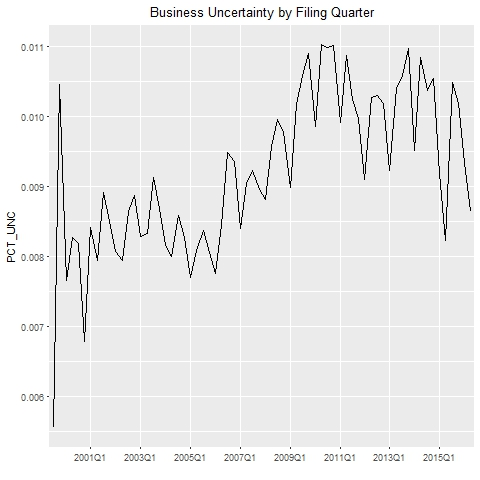
\includegraphics[width=6in, height=3in]{figures/bunc-by-quarter}
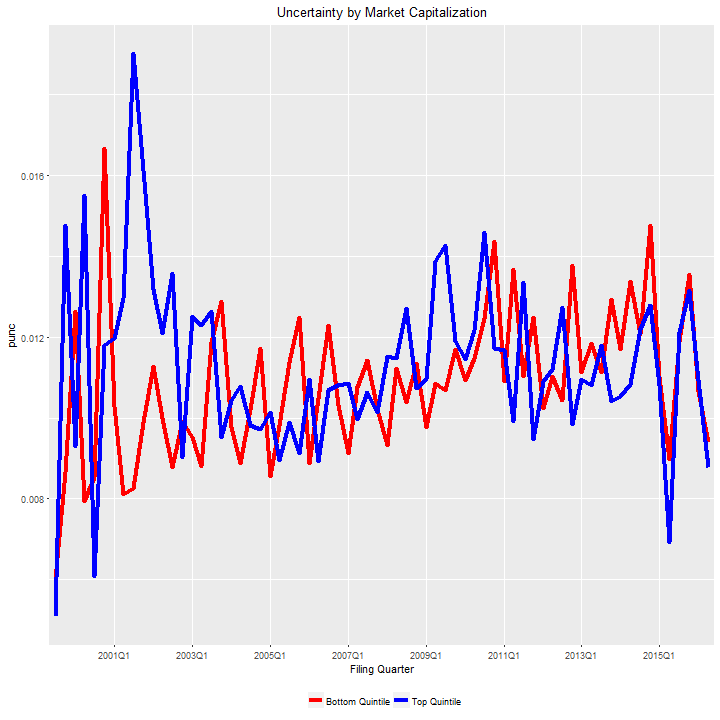
\includegraphics[width=6in, height=3in]{figures/bunc-by-mve}
\captionsetup{justification=centering, width=.95\textwidth} 
\caption{\footnotesize (Top panel) Time series trends of uncertainty} \label{bunc-figures}
\end{figure} 
\newpage
% TS and XS Total Assets
\begin{figure}[H] 
\centering
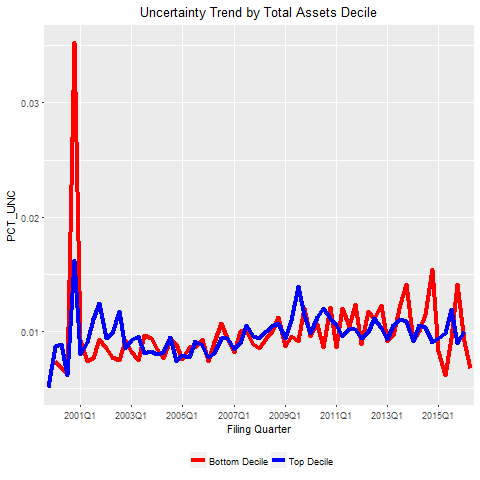
\includegraphics[width=3in, height=3in]{figures/punc-by-at-ts}
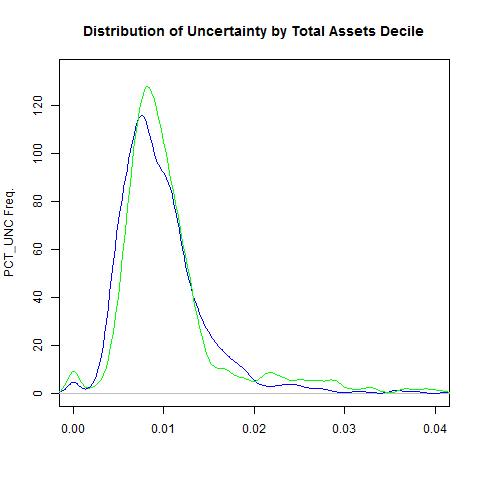
\includegraphics[width=3in, height=3in]{figures/punc-by-at-xs}
\captionsetup{justification=centering, width=.95\textwidth} 
\caption{\footnotesize Time series trends (left) and cross-sectional distribution (right) of uncertainty by total assets quintile.} \label{bunc-at}
\end{figure} 
% TS and XS Market-to-Book
\begin{figure}[H] 
\centering
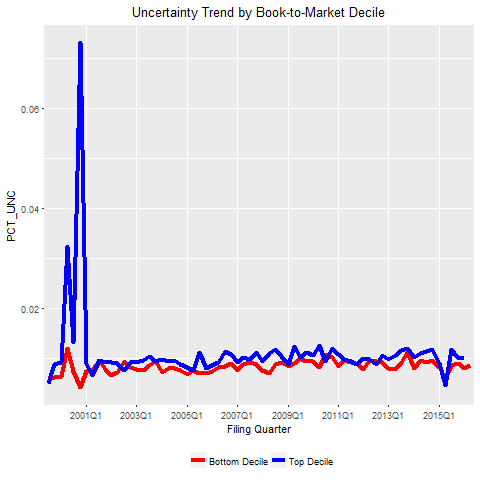
\includegraphics[width=3in, height=3in]{figures/punc-by-bm-ts}
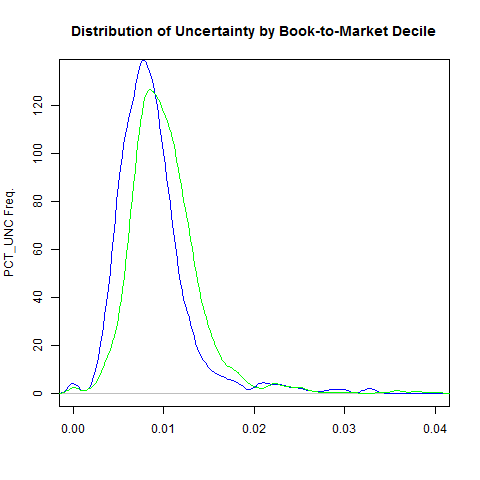
\includegraphics[width=3in, height=3in]{figures/punc-by-bm-xs}
\captionsetup{justification=centering, width=.95\textwidth} 
\caption{\footnotesize Time series trends (left) and cross-sectional distribution (right) of uncertainty by book-to-market quintile.} \label{bunc-bm}
\end{figure} 
\newpage
% TS and XS Tangibility
\begin{figure}[H] 
\centering
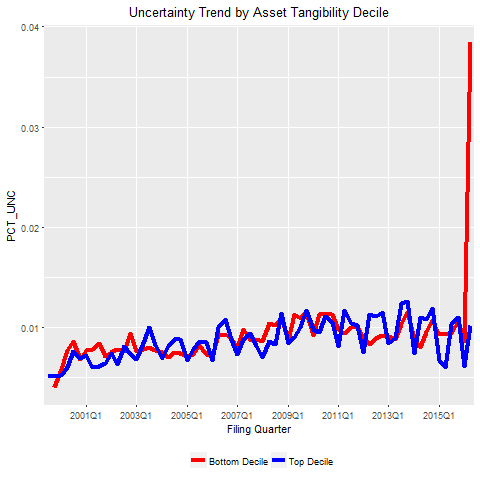
\includegraphics[width=3in, height=3in]{figures/punc-by-tang-ts}
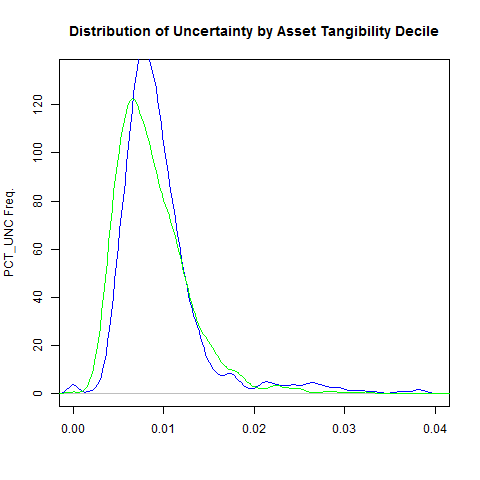
\includegraphics[width=3in, height=3in]{figures/punc-by-tang-xs}
\captionsetup{justification=centering, width=.95\textwidth} 
\caption{\footnotesize Time series trends (left) and cross-sectional distribution (right) of uncertainty by asset tangibility quintile.} \label{bunc-tang}
\end{figure} 
% TS and XS Forward PE
\begin{figure}[H] 
\centering
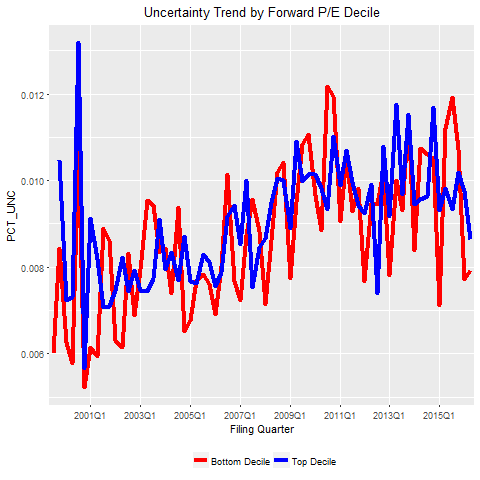
\includegraphics[width=3in, height=3in]{figures/punc-by-pefwd-ts}
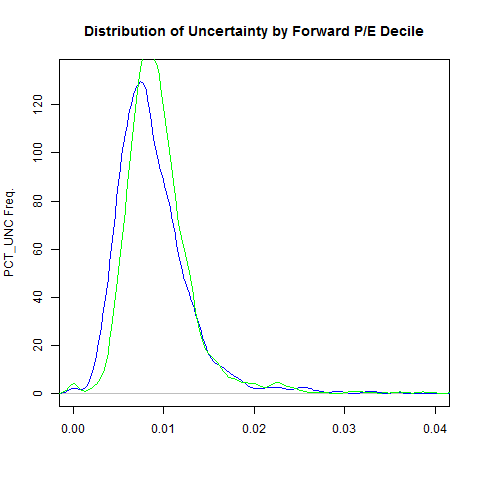
\includegraphics[width=3in, height=3in]{figures/punc-by-pefwd-xs}
\captionsetup{justification=centering, width=.95\textwidth} 
\caption{\footnotesize Time series trends (left) and cross-sectional distribution (right) of uncertainty by forward PE quintile.} \label{bunc-pefwd}
\end{figure} 
\newpage
% TS and XS Price
\begin{figure}[H] 
\centering
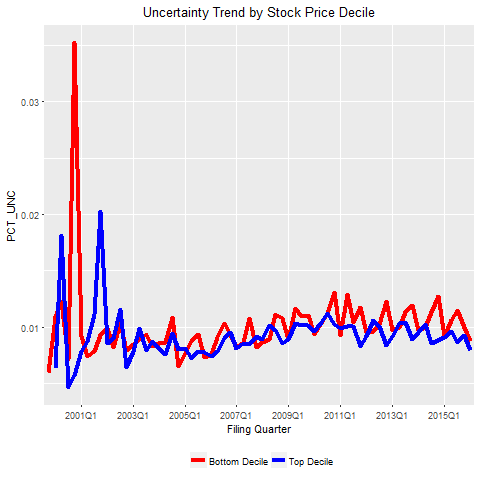
\includegraphics[width=3in, height=3in]{figures/punc-by-price-ts}
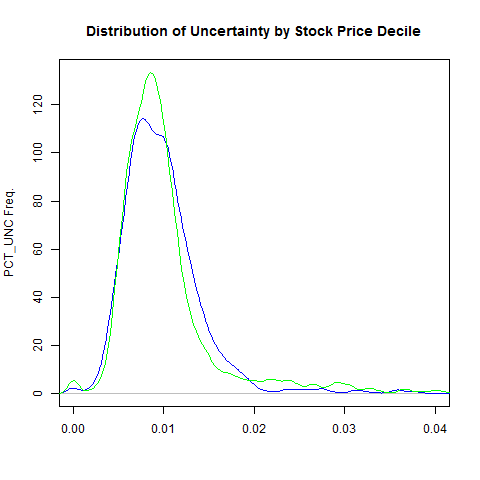
\includegraphics[width=3in, height=3in]{figures/punc-by-price-xs}
\captionsetup{justification=centering, width=.95\textwidth} 
\caption{\footnotesize Time series trends (left) and cross-sectional distribution (right) of uncertainty by stock price quintile.} \label{bunc-price}
\end{figure} 
% TS and XS Returns
\begin{figure}[H] 
\centering
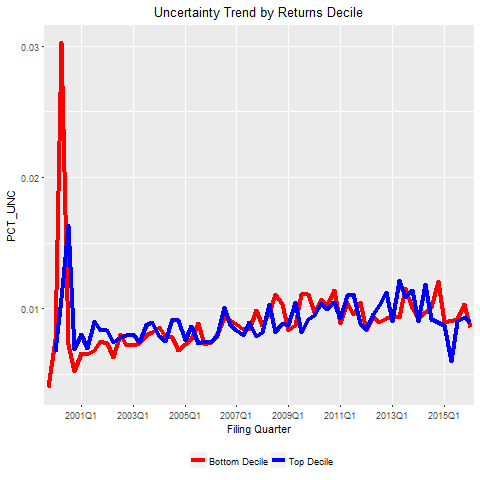
\includegraphics[width=3in, height=3in]{figures/punc-by-bhr-ts}
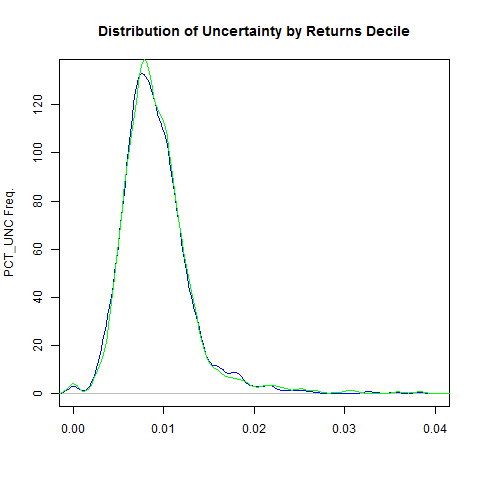
\includegraphics[width=3in, height=3in]{figures/punc-by-bhr-xs}
\captionsetup{justification=centering, width=.95\textwidth} 
\caption{\footnotesize Time series trends (left) and cross-sectional distribution (right) of uncertainty by stock returns quintile.} \label{bunc-bhr}
\end{figure} 
\newpage
% TS and XS Turnover
\begin{figure}[H] 
\centering
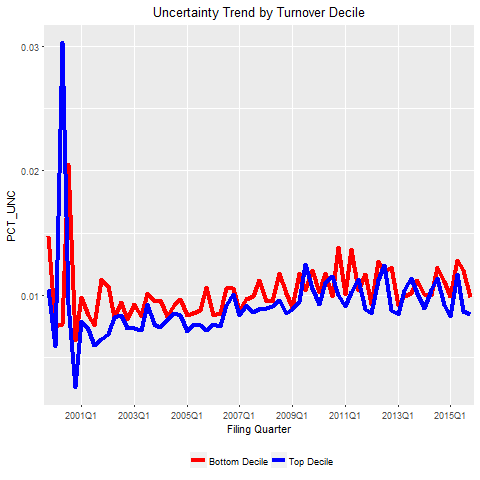
\includegraphics[width=3in, height=3in]{figures/punc-by-turn-ts}
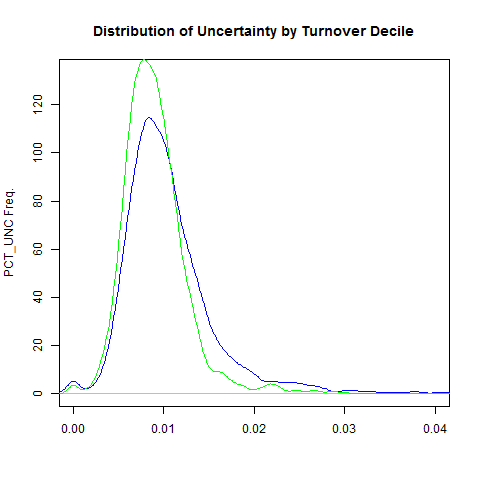
\includegraphics[width=3in, height=3in]{figures/punc-by-turn-xs}
\captionsetup{justification=centering, width=.95\textwidth} 
\caption{\footnotesize Time series trends (left) and cross-sectional distribution (right) of uncertainty by stock turnover quintile.} \label{bunc-turn}
\end{figure} 
\newpage
% TS and XS NANALYSTS
\begin{figure}[H] 
\centering
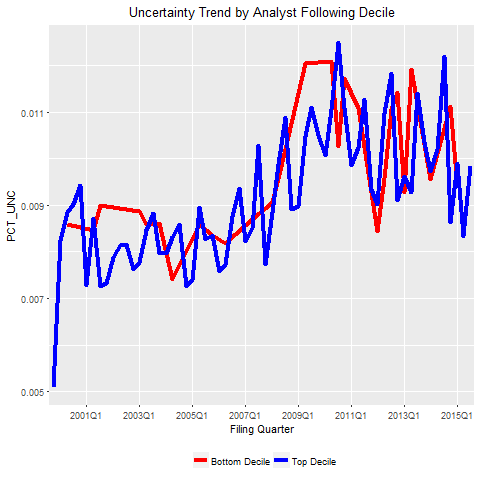
\includegraphics[width=3in, height=3in]{figures/punc-by-nanalysts-ts}
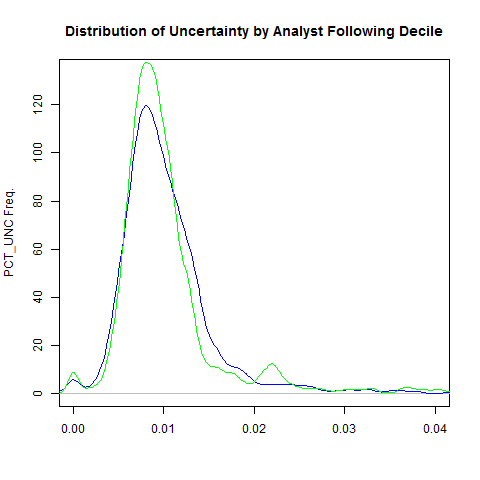
\includegraphics[width=3in, height=3in]{figures/punc-by-nanalysts-xs}
\captionsetup{justification=centering, width=.95\textwidth} 
\caption{\footnotesize Time series trends (left) and cross-sectional distribution (right) of uncertainty by analyst following quintile.} \label{bunc-nanalysts}
\end{figure} 
% TS and XS Analyst Dispersion
\begin{figure}[H] 
\centering
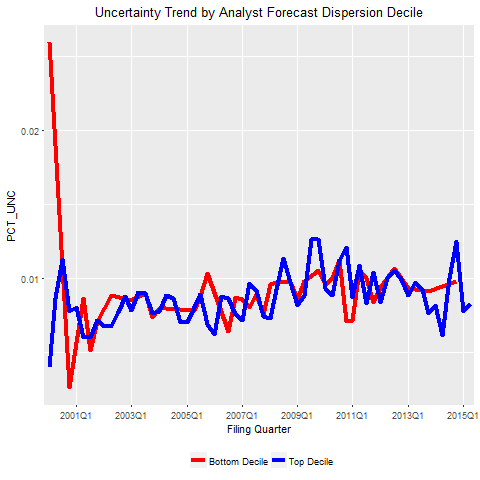
\includegraphics[width=3in, height=3in]{figures/punc-by-dispersion-ts}
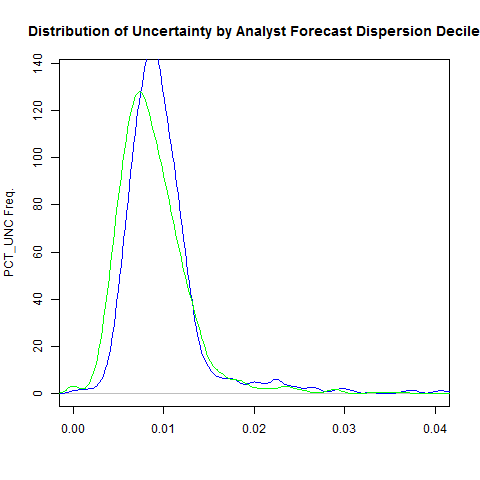
\includegraphics[width=3in, height=3in]{figures/punc-by-dispersion-xs}
\captionsetup{justification=centering, width=.95\textwidth} 
\caption{\footnotesize Time series trends (left) and cross-sectional distribution (right) of uncertainty by analyst forecast dispersion quintile.} \label{bunc-disp}
\end{figure} 
\newpage
%% Time series plots of aggregates
%%ROA
\begin{figure}[H] 
\centering
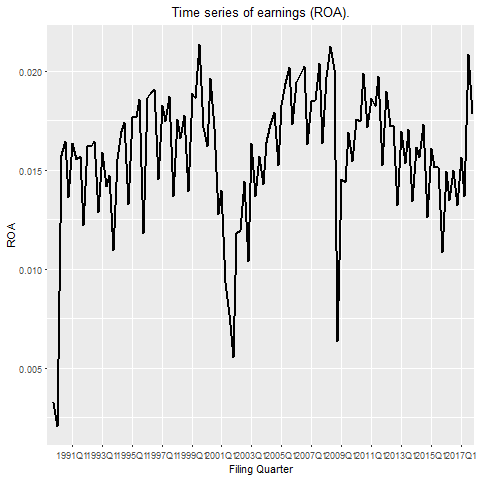
\includegraphics[width=5in, height=2.66in]{figures/roa-ts}
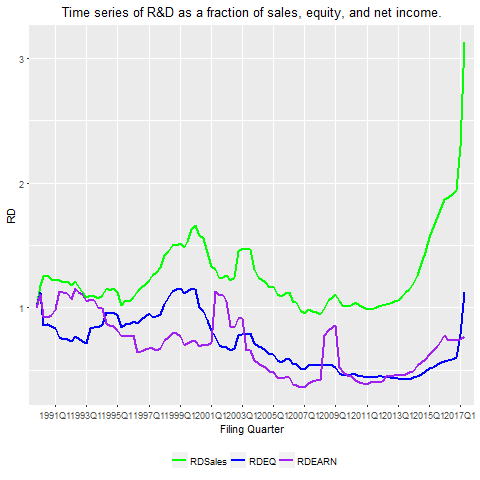
\includegraphics[width=5in, height=2.66in]{figures/rd-ts}
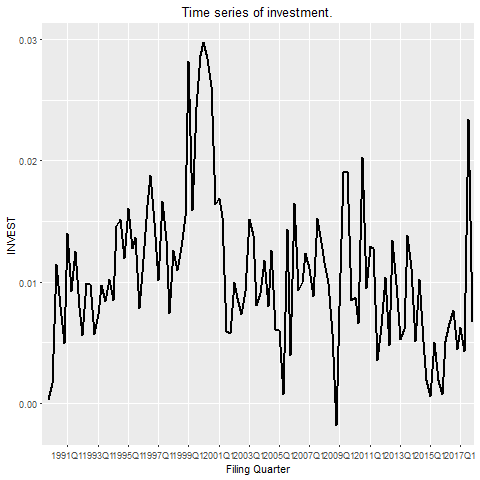
\includegraphics[width=5in, height=2.66in]{figures/invest-ts}
\captionsetup{justification=centering, width=.95\textwidth} 
\caption{\footnotesize Time series trends of Earnings, R\&D, and Investment} \label{ts-plots}
\end{figure} 
 \newpage 

%%ACF and PACF Plots: ROA
\begin{figure}[H] 
\centering
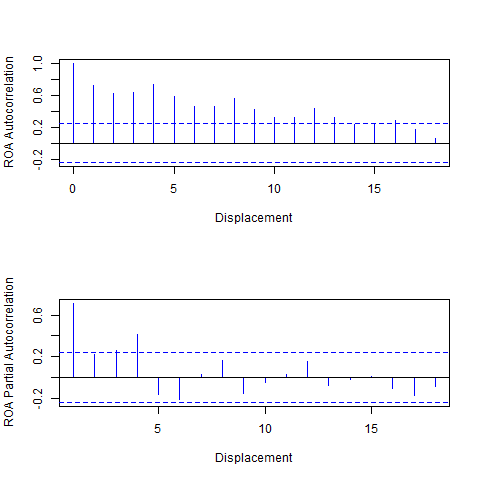
\includegraphics[width=5in, height=6in]{figures/roa-acf}
\captionsetup{justification=centering, width=.95\textwidth} 
\caption{\footnotesize Earnings (ROA) sample autocorrelation and partial autocorellation functions.} \label{roa-acf}
\end{figure} 
 \newpage 

%%ACF and PACF Plots: Investment
\begin{figure}[H] 
\centering
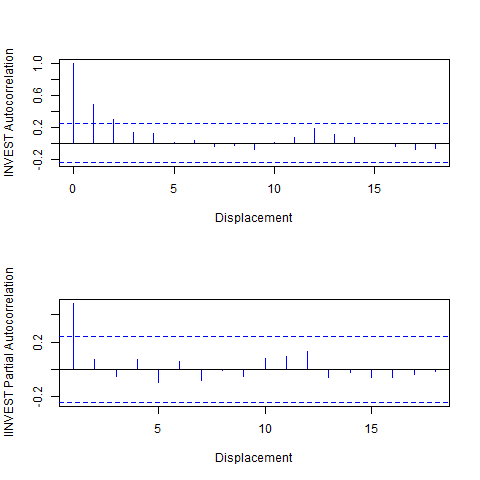
\includegraphics[width=5in, height=6in]{figures/invest-acf}
\captionsetup{justification=centering, width=.95\textwidth} 
\caption{\footnotesize Investment sample autocorrelation and partial autocorellation functions.} \label{invest-acf}
\end{figure} 
 \newpage 

%%ACF and PACF Plots: RD
\begin{figure}[H] 
\centering
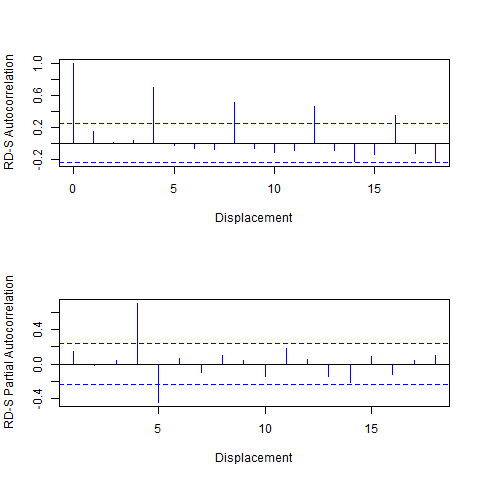
\includegraphics[width=5in, height=6in]{figures/rdsales-acf}
\captionsetup{justification=centering, width=.95\textwidth} 
\caption{\footnotesize R\&D sample autocorrelation and partial autocorellation functions.} \label{rd-acf}
\end{figure} 
 \newpage

%% VAR
\begin{figure}[H] 
\centering
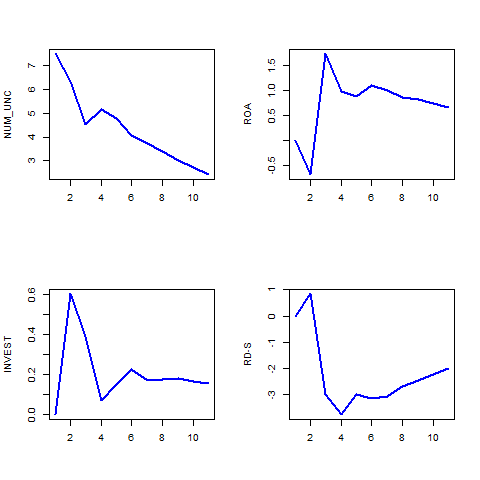
\includegraphics[width=6in, height=6in]{figures/nunc-irf-2}
\captionsetup{justification=centering, width=.95\textwidth} 
\caption{\footnotesize Impulse-Response Functions for $NUM\_UNC$.} \label{nunc-irf-2}
\end{figure} 
 \newpage
\begin{figure}[H] 
\centering
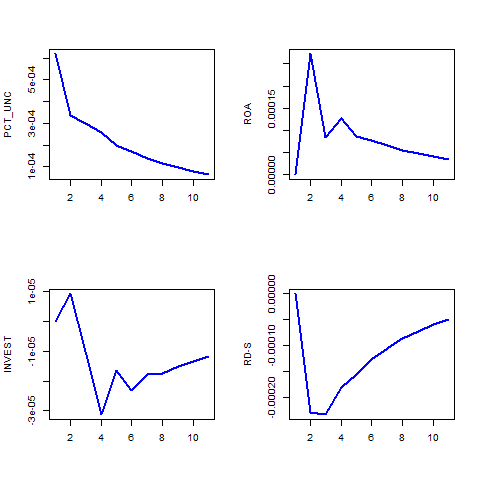
\includegraphics[width=6in, height=6in]{figures/punc-irf-2}
\captionsetup{justification=centering, width=.95\textwidth} 
\caption{\footnotesize Impulse-Response Functions for $PCT\_UNC$.} \label{punc-irf-2}
\end{figure} 
 \newpage
%% CCF Plots
\begin{figure}[H] 
\centering
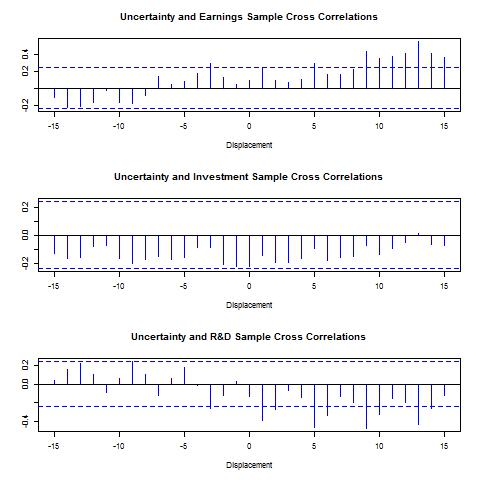
\includegraphics[width=6in, height=8in]{figures/ccf}
\captionsetup{justification=centering, width=.95\textwidth} 
\caption{\footnotesize Sample Cross-Correlation Plots} \label{ccf-plots}
\end{figure} 
